\documentclass[12pt]{article}
\usepackage[a4paper, margin=.30in]{geometry}
\usepackage{graphicx ,
            wrapfig,
            xcolor, 
            enumerate,
            amsmath,fontenc
            }
\usepackage{mathptmx}

\newcommand\headerMe[2]{\noindent{}#1\hfill#2}
\renewcommand{\thesection}{\Roman{section}}

\author{Zakaria HAOUZAN}
\date{\today}

\begin{document}
% headers --------------
\headerMe{Matière : Physique-Chimie}{Professeur : Zakaria HAOUZAN}\\
\headerMe{Unité : Electricité}{Établissement : Lycée SKHOR qualifiant}\\
\headerMe{Niveau : 1BAC-SM}{Heure : 5H}\\

% ------Content ________
\begin{center}

    \Large{Leçon $N^{\circ} 6 $: \color{red}Le champ électrostatique (Sc.Math) }
\end{center}

%\begin{wrapfigure}[10]{r}{0.5\textwidth}
    %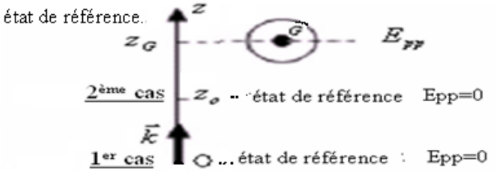
\includegraphics[width=0.5\textwidth]{./img/img00.png}
%\end{wrapfigure}

\section{notion de Champ électrostatique:}
\subsection{Expérience :}
En électrisant la boule d’un pendule électrostatique à l’aide d’un bâton d’ébonite électrisé par frottement puis en lui approchant
un bâton de verre chargé positivement par frottement. , on constate que le pendule s’incline et la boule prend une position après avoir
être attirée vers le bâton.
\begin{center}
    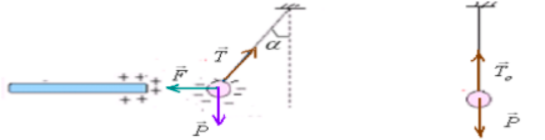
\includegraphics[width=0.5\textwidth]{./img/img_00.png}
\end{center}
\subsection{Interprétation : }
Dans la 1ère position d’équilibre, le pendule est vertical, la boule se trouve seulement dans le champ de pesanteur : $\vec{P} + \vec{T} = \vec{0}$

Dans la 2ème position d’équilibre, le pendule est incliné, la boule se trouve en plus du champ de pesanteur dans un autre champ
appelée: le champ électrostatique dans lequel les charges positives du bâton appliquent une force appelée : force électrostatique
sur les charges négatives de la boule du pendule.
Dans ce dernier cas la condition d’équilibre s’écrit :$\vec{P} +\vec{F} + \vec{T} = \vec{0}$
\begin{center}
    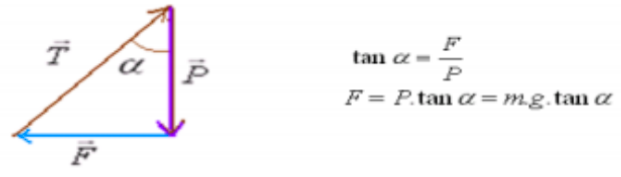
\includegraphics[width=0.5\textwidth]{./img/img_01.png}
\end{center}

\subsection{Conclusion : }
Dans une région de l’espace la charge électrique crée autour d’elle un champ électrique et tout corps chargé qui se trouve en un
point de ce champ, est soumis à une force électrique.

\subsection{Enoncé de la loi de Coulomb :}
Le physicien français Coulomb a étudié les interactions électrostatiques et il a réalisé une expérience avec la balance de torsion en
1785 lui permettant de formuler la loi d’attraction et de la répulsion qui a pris son nom.

Deux corps A et B de charges qA et qB s'attirent ou se repoussent selon une force proportionnelle à leur charge et inversement
proportionnelle au carré de la distance qui les sépare.

Les deux forces on :  même droite d'action et de sens opposés - même intensité.
$$F_{A/B} = F_{B/A} = K.\frac{q_A.q_B}{r^2}$$
avec : $K = \frac{1}{4\pi.\epsilon_0} N.m^2/C^2$ et$ \epsilon_0$ : permittivité du vide , sa valeur : $\epsilon_0 = \frac{1}{36.10^9\pi}=8.84SI $
\begin{center}
    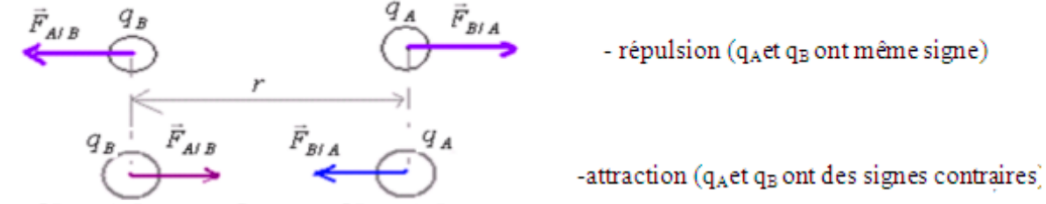
\includegraphics[width=0.5\textwidth]{./img/img_02.png}
\end{center}

\section{ Champ électrique/force électrique }
\subsection{Champ électrique créé par une charge ponctuelle :}
Une charge ponctuelle Q, placé en un point A crée un champ électrique dans l’espace qui l’entour. En un point M de cet espace
) où règne le champ électrique ( une charges q est soumise à une forces électrique : $\vec{F} = K.\frac{Q_A.q_B}{r^2}.\vec{u}$ qui est de la forme$\vec{F} = q_B.\vec{E}$ Le vecteur champ électrique créé par la charge Q au point M tel que : $\vec{E} = k.frac{Q}{r^2}.\vec{u}$
\begin{center}
    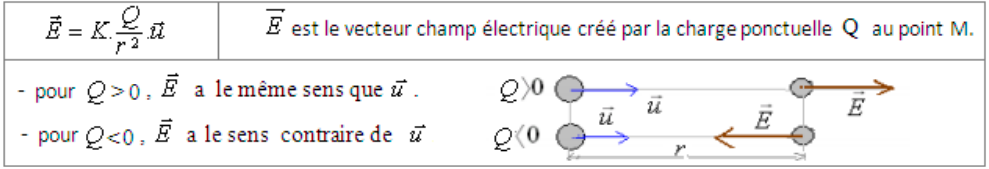
\includegraphics[width=0.8\textwidth]{./img/img_03.png}
\end{center}
Remarquons que c’est la charge Q qui a créé le champ électrique alors que q a subit la force électrique (car elle est placé dans le
 champ électrique).
 Toute charge immobile crée autour d’elle un champ électrique dont le vecteur champ
$\vec{E}$ en un point M du champ est centripète si la charge (qui crée le champ) est négative et centrifuge si elle est positive.
\begin{center}
    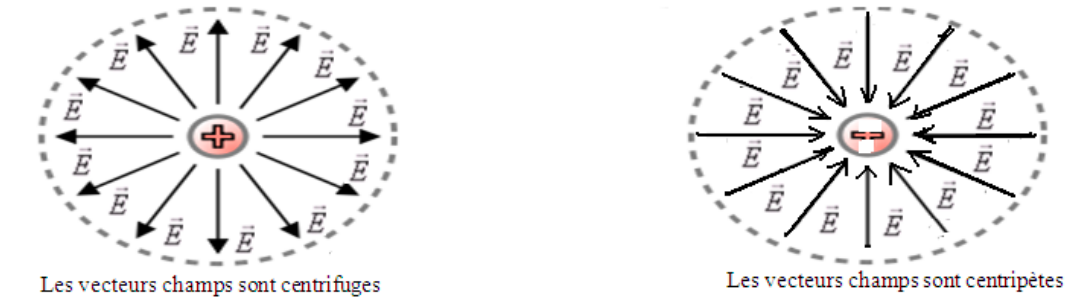
\includegraphics[width=0.8\textwidth]{./img/img_04.png}
\end{center}

\subsection{Force électrique : }
Toute charge q placé dans un champ électrique $\vec{E}$  est soumise à une force électrique $\vec{F}$ d’intensité: $F = q.E$ 
\begin{itemize}
      \item F en N
      \item q en C
      \item E en (V/m) ou (N/C)
\end{itemize}
La force électrique $\vec{F} = q\vec{E}$ : Si $q>0$ $\vec{F}$ a le même sens que $\vec{E }$  ;Si $q<0$ $\vec{F}$ a le même contraire de $\vec{E}$

\subsection{Champ électrique créé par deux charges ponctuelles:}
Considérons deux charges ponctuelles : $q_1>0 et q_2<0$ placée respectivement aux point A et B et un point M qui n’appartient pas
à la ligne AB.
\begin{center}
    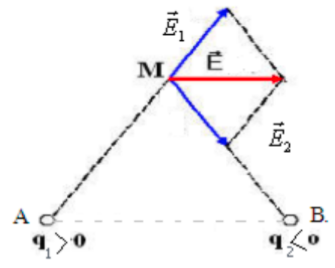
\includegraphics[width=0.3\textwidth]{./img/img_05.png}
\end{center}



Le vecteur champ électrique résultant $\vec{E}$ créé par les deux charges au point M est égale à la somme des deux vecteurs $\vec{E_1} et 
\vec{E_2}$

Généralisation :
Le vecteur champ électrique créé par un ensemble de charges électriques ponctuelles est égale à la somme des champs électriques
créé par chaque charge électrique .

\subsection{Lignes de Champ électrique : }
On appelle ligne de champ la ligne qui , en chacun de ses points, est tangente au vecteur champ électrique $\vec{E}$.les lignes de champ
sont orienté dans le sens du vecteur champ électrique.

\begin{center}
    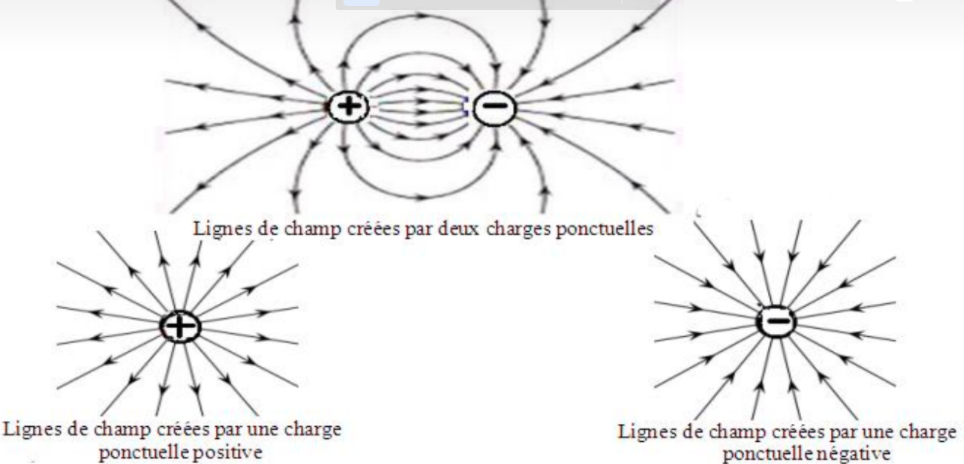
\includegraphics[width=0.7\textwidth]{./img/img_06.png}
\end{center}

\section{Champ électrique uniforme :}

\section{ Définition :}
Un champ électrique est dit uniforme dans une région de l'espace si le vecteur champ conserve en tout point de cette région, la même
direction, le même sens et la même valeur.
\section{Exemple : }
Entre deux plaques métalliques parallèles soumises à une différence de potentielle existe un champ électrique uniforme

\begin{itemize}
      \item VA : potentiel de la plaque A .
      \item VB : potentiel de la plaque B .
      \item d : distance entre les deux plaques
      \item Entre les deux plaques le champ électrique est uniforme .
      \item Les lignes de champ sont parallèles entre elles et perpendiculaires aux plans des plaques .
         \item Le vecteur champ électrique $\vec{E}$a le sens des potentiels décroissants c'est-à-dire de la plaque ayant le plus grand potentiel vers celle ayant le plus petit potentiel.
         \item La norme du champ électrique $\vec{E}$ entre les plaques  $E = \frac{U_AB}{d}$ en  V/m avec $U_AB = V_A-V_B$
\end{itemize}

\begin{center}
    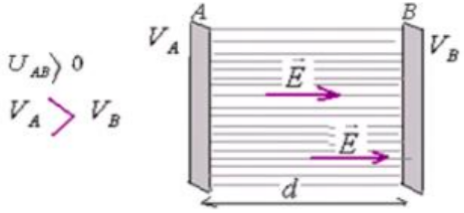
\includegraphics[width=0.4\textwidth]{./img/img_07.png}
\end{center}










\end{document}

